\documentclass[12pt]{article}

%-------------------------------------------------
%   THEMES & PACKAGES
%-------------------------------------------------
\usepackage{fancyhdr}
\usepackage{lastpage}
\usepackage{xcolor}
\usepackage{pdfpages}
\usepackage{hyperref}
\usepackage{graphicx}
\usepackage{enumitem}

%%% Custom colors & commands
\newcommand{\HRule}[1]{\rule{\linewidth}{#1}}   % Horizontal rule

%-------------------------------------------------
%   COMMON INFO
%-------------------------------------------------
\newcommand{\hmwkTitle}{R \& D Proposal}
\newcommand{\hmwkTopic}{Detecting Outliers in Physiological Data for Modeling Cardiovascular Response in Sport Exercises}
\newcommand{\hmwkDueDate}{May 15, 2016}
\newcommand{\hmwkClass}{Research and Development}
\newcommand{\hmwkAuthorName}{Minh H. Nguyen}
\newcommand{\hmwkAuthorSchool}{Bonn-Rhein-Sieg University of Applied Sciences}
\newcommand{\hmwkAdvisorFirst}{Prof. Dr. Erwin Prassler}
\newcommand{\hmwkAdvisorSecond}{Matthias F{\"u}ller}

\graphicspath{{../images/}}

%-------------------------------------------------
%   MARGINS
%-------------------------------------------------
\topmargin=-0.75cm
\evensidemargin=0cm
\oddsidemargin=0cm
\textwidth=16.0cm
\textheight=22.0cm
\headsep=0.6cm

\linespread{1.1} % Line spacing

%-------------------------------------------------
%   HEADERS & FOOTERS
%-------------------------------------------------
\pagestyle{fancy}
%-------------------------------------------------
% Special first page
\fancypagestyle{firststyle} {
    \fancyhf{}
    \fancyfoot{}
    \renewcommand\headrulewidth{0.pt}
    \renewcommand\footrulewidth{0.pt}
}
%-------------------------------------------------
\lhead{\hmwkAuthorName}
\rhead{\hmwkTitle}
%-------------------------------------------------
\cfoot{Page \thepage\ of \protect\pageref{LastPage}}
%-------------------------------------------------
\renewcommand\headrulewidth{0.4pt}
\renewcommand\footrulewidth{0.4pt}

%-------------------------------------------------
%   TITLE
%-------------------------------------------------
\title{\normalsize \textsc{\hmwkAuthorSchool}   % Subtitle
    \\[2.0cm]                                   % 2cm spacing
    \HRule{0.5pt} \\                            % Upper rule
    \LARGE \textbf{\uppercase{\hmwkTopic}}
    \HRule{2pt} \\ [0.5cm]                      % Lower rule + 0.5cm spacing
    \hmwkTitle\\[0.5cm]
    \normalsize \hmwkDueDate\\
}

\author{
    \\[4.0cm]
    Author:\\
    \hmwkAuthorName\\
    \ \\
    Advisors:\\
    \hmwkAdvisorFirst\\
    \hmwkAdvisorSecond\\
}

\date{}

%-------------------------------------------------
%   BIBLIOGRAPHY
%-------------------------------------------------
\usepackage[english]{babel}
\usepackage[backend=biber]{biblatex}
\addbibresource{../RnD.bib}
\addbibresource{proposal.bib}

%-------------------------------------------------
%   BEGIN
%-------------------------------------------------
\begin{document}
%-------------------------------------------------
    \maketitle
    \thispagestyle{firststyle}
    \newpage

%-------------------------------------------------
\section{Introduction}

    %---------------------------------------------
    \subsection{Motivation}

    Significance of heart rate prediction:
    \begin{itemize}
        \item Health benefits of exercise can be improved by better understanding of how the heart react to different forms of physical exertion.
        \item Machine learning has shown promising results in modeling heart rates for running exercises \autocite{Fueller2015}
    \end{itemize}

    Physiological data recorded using \underline{hand-held} (better term?) devices (i.e. the Polar H7 sensor) can sometimes contain invalid data due to low battery level, external electromagnetic influences \underline{(citation needed)}.
    \begin{itemize}
        \item Such unreliability can impair generalization ability of heart rate modeling techniques \underline{(citation needed)}
        \item Automatic removal of such outliers in the larger datasets can improve performance of existing models.
        \item Anomaly models for temporal data can vary greatly depending on the specific data type and scenario, therefore need to be designed for the particular problem \autocite{Gupta2013}.
    \end{itemize}

    This project aims to survey existing outlier detection techniques for temporal data, to find a suitable outlier model for physiological data used in the heart rate prediction task.

    %---------------------------------------------
    \subsection{Prior Work}
    \begin{figure}[h!]
        \centering
        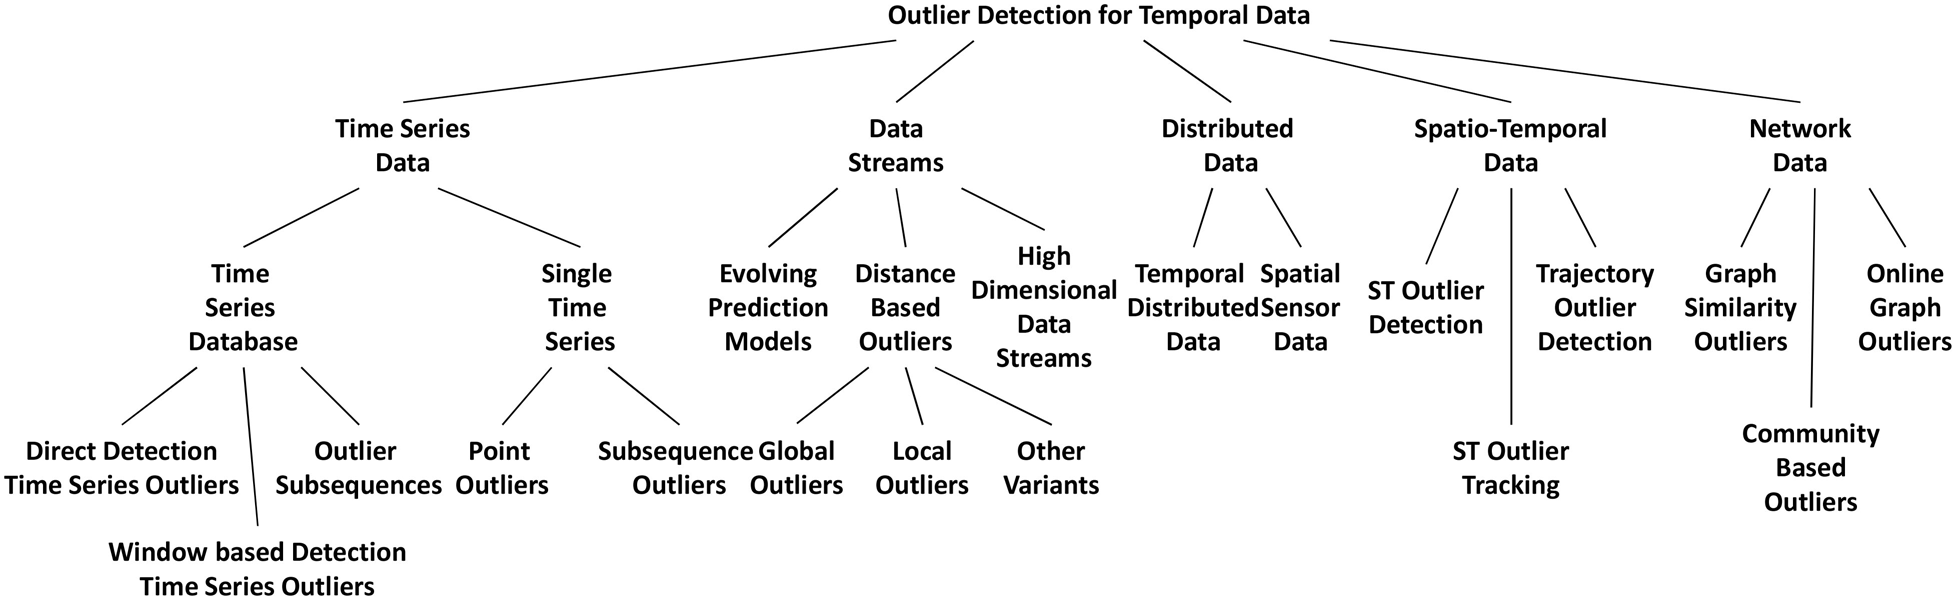
\includegraphics[width=0.9\linewidth]{gupta2014-mind_map.png}
        \caption{Outlier detection mind map \autocite{Gupta2013}}
        \label{fig:mindmap}
    \end{figure}
    Detecting anomaly in temporal data can involve a wide variety of tasks as shown in the mind map in figure \ref{fig:mindmap} proposed by Gupta et al. For the heart rate prediction task, outlier models for time series are most relevant. Since the data set contains a large number of relatively short time series, this paper will focus on finding anomalies in the whole database, as opposed to abnormalities within individual time series.

    Following the categorization by Gupta et al., detection of abnormal time series sequences within a database can be done directly, through identifying anomalous time windows or through finding outlier subsequences in a test time series.
    \subsubsection{Direct detection}
    \subsubsection{Window-based detection}
    \subsubsection{Outlier subsequence detection}

    %---------------------------------------------
    \subsection{Approach}


    %---------------------------------------------
    \subsection{Expected Results}


%-------------------------------------------------
\section{Project Plan}

    %---------------------------------------------
    \subsection{Work Packages}

    %---------------------------------------------
    \subsection{Work Schedule}
    %\includepdf[pages={1}]{rnd_nguyen_workschedule_gannt.pdf}

\printbibliography

%-------------------------------------------------
%   END
%-------------------------------------------------
\end{document}
